\section{Introduction}
Institutional portfolios are increasingly built by optimizers. An objective
such as portfolio yield is maximized subject to a mandate: limits on exposure
to any single issuer, a ceiling on interest-rate risk, a floor on average
credit quality. The solver returns an allocation but not a reason that a
portfolio manager, client or examiner can read. A natural shortcut is to ask a
large language model (LLM) to explain the allocation. LLMs write fluent and
confident explanations, and the question is whether those explanations are
\emph{true}.

The interpretability literature separates an explanation that is
\emph{plausible} from one that is \emph{faithful} to the process that produced
the decision~\cite{jacovi20,lyu24}, and documents that LLM explanations are
often plausible but unfaithful~\cite{turpin23,matton25}. Testing faithfulness is
hard when the decision-maker is a neural model. One must intervene on the cause
an explanation names and see whether the decision moves, and the effect of
that intervention can only be estimated~\cite{atanasova23,zaman25}.

Linear programming is a setting where the test can be exact. The solver's
optimality certificate states which constraints bind and the marginal value
(shadow price) of relaxing each one~\cite{bertsimas97}. A claim of the form
``limit $i$ drove the allocation and is worth about $x$ basis points'' can
therefore be checked by relaxing limit $i$ and re-solving. If the optimum does
not move, the limit did not drive the decision and the claim is false, however
persuasive the surrounding prose. Exact oracles have recently been used to
grade LLM explainers of sequential decision policies~\cite{gross26}, and
solver-grounded LLM assistants exist for optimization
models~\cite{optiguide23,optichat25}. We use the linear-programming certificate
to measure, claim by claim, how faithfully two widely used commercial LLMs
explain constrained portfolio decisions when they reason from the solution
alone, without access to the certificate.

Our contributions are as follows.
\begin{enumerate}\itemsep1pt
\item A claim-level test for free-form explanations of linear-programming
allocation decisions. It separates attribution to limits whose effect is
exactly zero from error in the stated magnitudes. The first classification is
exact because the optimal value is concave in each limit (\S\ref{sec:method}).
\item An evaluation on \nProblems{} bond-portfolio problems built from public
FRED data. We compare explanations read from the certificate, a fixed
template, and two LLMs with and without the portfolio facts that reveal which
limits are tight (\S\ref{sec:setup} and \S\ref{sec:results}).
\item Evidence that both LLMs cite limits with no effect in most of the cases
where that error is possible, name binding and non-binding limits at similar
rates, are not reliably corrected by being given the relevant facts, and
misstate magnitudes with biases in the same direction for both vendors
(\S\ref{sec:results}).
\end{enumerate}
We do not propose a new optimizer or explanation system, and our exactness
results apply to linear programs only.

\section{Related Work}
\label{sec:related}
\textbf{Faithfulness of explanations.} Faithfulness, meaning whether an
explanation reflects the reasoning actually used, is distinguished from
plausibility~\cite{jacovi20,lyu24}. Intervention-based tests judge an
explanation unfaithful when changing an input in a way that changes the
prediction is not reflected in the explanation~\cite{atanasova23}.
Simulatability asks whether an explanation lets an observer predict the
model~\cite{doshi17}. Recent work treats faithfulness causally~\cite{zaman25},
estimates the causal effect of the concepts an LLM's explanation
cites~\cite{matton25}, and tests the necessity and sufficiency of the factors an
LLM names for its own decisions, including in a financial-advisory
setting~\cite{pawar26}. Chain-of-thought explanations have been shown to
misstate the true reason for an answer~\cite{turpin23}. In these studies the
model explains its own decision and the effect of an intervention is estimated.
Here the LLM explains another system's decision and the effect is computed.

\textbf{Exact oracles for LLM explanations.} The work closest in spirit is Gross
and Spieker~\cite{gross26}, who grade LLM explainers of Markov-decision-process
policies against probabilistic model checking, using queries such as which
action is optimal in a given state. We apply the same idea to
linear-programming allocation, where the oracle is the optimality certificate,
and we score the attributions and magnitudes an LLM volunteers in a free-form
explanation rather than its answers to targeted queries.

\textbf{Explainable optimization.} Sensitivity analysis and duality give the
classical account of why a solution is optimal~\cite{bertsimas97}. Recent work
formalizes counterfactual explanations for optimization-based
decisions~\cite{korikov21,cflp25}, uses linear-relaxation duals to attribute
decisions of learned combinatorial policies~\cite{cea26}, provides software for
post-optimality analysis~\cite{pyoptexplain26}, and argues that explanation
should become a first-class concern of operations research~\cite{explopt26}.
These works construct explanations from the model. We test explanations written
without it.

\textbf{LLMs for optimization and finance.} OptiGuide~\cite{optiguide23} and
OptiChat~\cite{optichat25} answer practitioners' questions about optimization
models by calling solver functions. In OptiChat's ablation, GPT-4.1 answered
none of the sensitivity questions correctly once those functions were
removed~\cite{optichat25}. EOR scores LLM explanations of operations-research
what-if changes with an LLM judge and with experts~\cite{eor25}. A separate
literature checks whether LLMs \emph{formulate} optimization models correctly,
using solver-assisted verification~\cite{verisimpl26}, multi-check
validation~\cite{trival26}, hallucination detection~\cite{optargus26} and
duality-based falsification tests~\cite{falsify26}. A correctly formulated model
can still be explained unfaithfully. Financial LLM benchmarks evaluate question
answering and reasoning~\cite{fintrade26}. Our contribution is to measure, for
portfolio allocation, what an LLM asserts about a solver's decision when it
reasons from the solution alone.

\section{Method}
\label{sec:method}
\subsection{Setup}
We consider portfolio programs
\begin{equation}
\begin{aligned}
\max_{x}\;\; & y^\top x\\
\text{s.t.}\;\; & d^\top x \le D,\;\; q^\top x \ge Q,\;\; \textstyle\sum_i x_i = 1,\;\; 0 \le x_i \le \kappa,
\end{aligned}
\label{eq:lp}
\end{equation}
where $x$ are portfolio weights, $y$ asset yields, $d$ durations, $q$
credit-quality scores, $D$ a duration ceiling, $Q$ a quality floor and $\kappa$ a
single-issuer cap. The three mandate limits $(\kappa, D, Q)$ are the candidate
reasons an explanation can cite.

\subsection{Ground truth by re-solving}
For each limit $c$ we relax its right-hand side by a step of $0.001$ in its own
units (0.1 percentage point of cap, 0.001 years of duration, 0.001 of quality),
re-solve with HiGHS~\cite{huangfu18}, and express the change in optimal yield in
basis points (bp) per stated unit: per $+1$ percentage point of cap, per $+0.1$
years of duration ceiling, and per $-0.01$ of quality floor. A limit is
classified as having zero effect if this change is below $10^{-6}$ bp.

The optimal value of a linear program is concave in each right-hand side. If
relaxing a limit leaves the optimum unchanged, its marginal value is therefore
zero for every smaller step as well, and the zero-effect classification is
exact up to solver tolerance. For a binding limit, the step effect equals the
certificate's shadow price unless the step crosses a breakpoint of the value
function, in which case it is smaller. In our problems the two agree within 1\%
for \compExactOne\% of binding limits, a difference far smaller than the errors
reported in \S\ref{sec:mag}. We use the re-solve rather than the reported duals
because it does not depend on reading the certificate correctly and remains
well defined at degenerate vertices.

\subsection{Explanations as checkable claims}
Every explainer returns a set of claims of the form ``limit $c$ drove the
allocation and relaxing it would add $\hat\lambda_c$ bp''. We score two things.
\begin{itemize}\itemsep1pt
\item \textbf{Zero-effect attribution:} over all (problem, limit) pairs where the
limit's effect is zero, the share in which the explainer named the limit as a
driver. This is the error most likely to mislead a reader, because it states a
reason that provably had no influence. It requires no units or tolerance.
\item \textbf{Magnitude accuracy:} over claims about limits whose effect is
non-zero, the share with $\hat\lambda_c$ within $\pm35\%$ of the true value.
\end{itemize}
We also report how often binding limits are named, which shows whether an
explainer discriminates between limits that matter and limits that do not, and
the explanation-level \emph{hard-failure rate}, the share of explanations naming
at least one zero-effect limit.

\subsection{Explainers}
\textbf{Certificate-grounded.} Reads the binding limits and their shadow prices
from the certificate and states them. It is correct by construction and serves
as a check that the scoring is calibrated, not as a finding.

\textbf{Template.} Always names the issuer cap and the duration ceiling with
fixed sizes of 10 and 5 bp. It shows what a constant answer achieves.

\textbf{LLM, basic.} The model sees the constraint limits, every held bond
(weight, yield, duration and quality) and the portfolio's yield, but not the
certificate. It is asked which limits shaped the allocation and how many basis
points relaxing each would add, in the units above, ending with a
machine-readable line. The prompt states that ``a constraint that is not tight
would gain 0 bp and is NOT a driver'' and asks the model to include a
constraint only if it believes relaxing it would raise yield
(Appendix~\ref{app:prompt}).

\textbf{LLM, with facts.} As above, plus the realized average duration and
average quality next to their limits, and the number of holdings at the cap.
These facts are sufficient to tell which limits are tight. The certificate is
still withheld.

\begin{figure}[t]
\centering
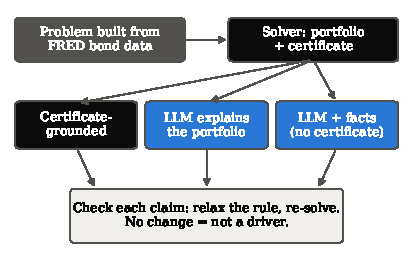
\includegraphics[width=\figw]{fig_v5_pipeline.pdf}
\caption{The test. Every claim made by an explainer is checked by relaxing the
named limit and re-solving the portfolio problem.}
\label{fig:pipeline}
\end{figure}

\section{Experimental Setup}
\label{sec:setup}
\textbf{Data.} We build asset universes from FRED~\cite{fredust,fredice}: US
Treasury constant-maturity yields at 1--30 years and ICE BofA US corporate
option-adjusted spreads for ratings AAA to CCC. Each asset is a representative
bond for one (rating, maturity) cell, with yield equal to the Treasury yield
plus the rating spread and duration equal to that of a par bond. Quality scores
map ratings to $[0,1]$. This gives 64 assets per date. We use six dates: the
month-ends of May to September 2026 and October 14, 2026.

\textbf{Problems.} Each problem samples 25--59 assets from one date's universe
and draws the three limits so that, across problems, the duration and quality
limits are sometimes tight and sometimes slack. With market spreads all three
limits bind in most problems (77 of 96 in our first set), which leaves few cases
that test zero-effect attribution. We therefore use two sets: a \emph{natural}
set (\nMain{} solvable problems, \nSlackCasesMain{} zero-effect cases) and a
\emph{slack-focused} set of \nSlack{} problems, each with at least one
zero-effect limit (\nSlackCasesSlack{} cases). The issuer cap bound in every
problem, so all zero-effect cases concern the duration ceiling (74) or the
quality floor (75). Every explainer sees the same problems. In \degMain{} and
\degSlack{} problems respectively, some limit's measured effect changed by more
than 25\% between steps of 0.0005 and 0.001, which indicates a breakpoint close
to the optimum. These problems are kept.

\textbf{Models.} Claude Sonnet~4.5 and Gemini~2.5 Flash were called through
OpenRouter in October 2026 at temperature 0, with one reply per problem and
prompt.\footnote{OpenRouter identifiers: \texttt{anthropic/\allowbreak claude-sonnet-4.5},
\texttt{google/\allowbreak gemini-2.5-flash} and \texttt{openai/\allowbreak gpt-4o-mini}.}
All replies could be parsed. A third model, GPT-4o-mini, was run in the same
way; \S\ref{sec:anchor} explains why it is reported separately.

\section{Results}
\label{sec:results}

\subsection{A worked example}
We chose the following problem to illustrate the error. It is from \exDate{}
(optimal yield \exObj\%). The certificate shows that the issuer cap and the
duration ceiling bind: relaxing the cap adds \exCapTrue{} bp per percentage point
and relaxing the duration ceiling adds \exDurTrue{} bp per 0.1 years. The quality
floor is not tight, and relaxing it adds nothing. Gemini~2.5 Flash, shown that
the portfolio's average quality is \exAvgQ{} against a floor of \exQFloor{},
answered that \emph{``the credit-quality floor is active, with the portfolio's
average quality score just above the 0.47 floor''} and valued it at
\exQualClaim{} bp. It valued the cap at \exCapClaim{} bp (true value \exCapTrue)
and the duration ceiling at \exDurClaim{} bp (true value \exDurTrue). Each
statement reads as reasonable. One names a limit with no effect, and the other
two are off by a factor of about seven.

\subsection{Attributing the decision to limits that did not matter}
Table~\ref{tab:main} and Figure~\ref{fig:slack} give the main result. Across
\nSlackCases{} zero-effect cases, Claude Sonnet~4.5 named the limit as a driver
in \snSonFf\% of cases (95\% CI \snSonFfLo--\snSonFfHi) and Gemini~2.5 Flash in
\snGemFf\% (\snGemFfLo--\snGemFfHi). The certificate-grounded explainer, as
expected by construction, did so in none (upper bound \snCGHi\%). A template
that always names the cap and the duration ceiling scores \snTmpl\%. This figure
reflects the mix of slack limits, since the template names every slack duration
ceiling and no slack quality floor.

\textbf{Discrimination.} Claude named binding limits in \bindSonFf\% of cases and
zero-effect limits in \snSonFf\%, and it named all three limits in
\allthreeSonFf\% of its explanations. With the facts, the two rates were
\bindSonInf\% and \snSonInf\%. Gemini with the facts named every binding limit
and \snGemInf\% of zero-effect ones, a partial separation. For comparison, the
certificate gives 100\% and 0\%, and the template \bindTmpl\% and \snTmpl\%.

\textbf{Effect of the facts.} Showing the models the facts that reveal which
limits are tight did not change Claude's zero-effect rate by more than chance
would explain (exact McNemar test on paired cases, $p=\mcnSon$), but it reduced
Gemini's ($p=\mcnGem$). With the facts, Gemini was no better than the fixed
template (\snGemInf\% against \snTmpl\%, $p=\mcnGemTmpl$). With the basic
prompt, Claude named zero-effect limits more often than Gemini ($p=\mcnSonGem$).
Because two zero-effect limits in the same problem are not independent, we also
report bootstrap intervals that resample whole problems: \cbSonFf\ for Claude,
\cbGemFf\ for Gemini and \cbGemInf\ for Gemini with the facts. The natural set,
which was not selected for slack limits, gives similar rates (Claude 25 of 26,
Gemini 17 of 26), although it contains only 26 cases.

\begin{table}[t]
\centering
\small
\caption{Zero-effect attribution (named / zero-effect cases) in each problem
set and pooled with Wilson 95\% interval; share of binding limits named; and
share of stated magnitudes within $\pm35\%$ of the true value.
$^{*}$GPT-4o-mini copied the prompt's example values (\S\ref{sec:anchor}).}
\label{tab:main}
\resizebox{\tabw}{!}{\begin{tabular}{@{}lccccc@{}}
\toprule
& \multicolumn{2}{c}{Zero-effect rules named} & Pooled & Binding rules & Size within \\
Explainer & natural & slack-focused & (95\% CI) & named & $\pm$35\% \\
\midrule
Certificate-grounded & 0/26 & 0/123 & 0\% [0, 3] & 100\% & 99.7\% \\
Template: always cap + duration & 13/26 & 61/123 & 50\% [42, 58] & 72\% & 3\% \\
\midrule
Claude Sonnet 4.5, basic & 25/26 & 107/123 & 89\% [82, 93] & 98\% & 9\% \\
Claude Sonnet 4.5, with facts & 23/26 & 105/123 & 86\% [79, 91] & 100\% & 8\% \\
Gemini 2.5 Flash, basic & 17/26 & 97/123 & 77\% [69, 83] & 90\% & 6\% \\
Gemini 2.5 Flash, with facts & 14/26 & 57/123 & 48\% [40, 56] & 100\% & 7\% \\
GPT-4o-mini$^{*}$, basic & 16/26 & 72/123 & 59\% [51, 67] & 72\% & 4\% \\
GPT-4o-mini$^{*}$, with facts & 12/26 & 43/123 & 37\% [30, 45] & 95\% & 9\% \\
\bottomrule
\end{tabular}
}
\end{table}

\begin{figure}[t]
\centering
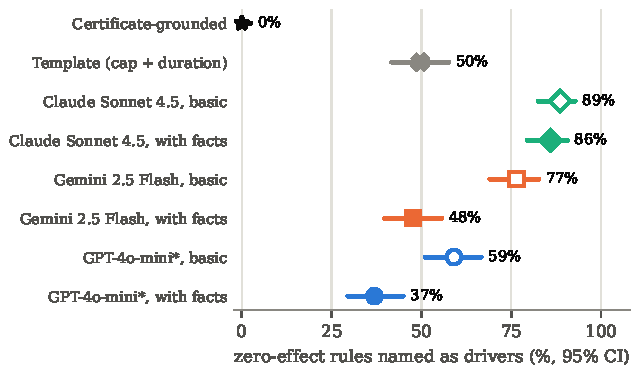
\includegraphics[width=\figw]{fig_v5_slack.pdf}
\caption{Share of zero-effect limits that each explainer named as a driver
(pooled over \nSlackCases{} cases; 95\% Wilson intervals). Open markers: basic
prompt; filled markers: with portfolio facts. $^{*}$See \S\ref{sec:anchor}.}
\label{fig:slack}
\end{figure}

\subsection{Misstating how much a limit costs}
\label{sec:mag}
For limits that did bind, the models' stated magnitudes were within $\pm35\%$ of
the true value in \magMain\% of \nMagMain{} claims (certificate: \magCG\%). The
errors run in the same direction for both vendors (Figure~\ref{fig:mag}). The
issuer cap is understated (median ratio of claimed to true value
$\ratioMainCap\times$), the duration ceiling is overstated
($\ratioMainDur\times$), and the quality floor is overstated
($\ratioMainQual\times$). The result does not depend on the tolerance: \tolTwenty\%,
\tolFifty\% and \tolTwoX\% of claims fall within $\pm20\%$, $\pm50\%$ and a factor of
two.

The information needed to compute these values is in the prompt. Held bonds
strictly between zero and the cap satisfy $y_j = \mu + \lambda_D d_j - \lambda_Q
q_j$, where $\mu$ is the budget multiplier and $\lambda_D$ and $\lambda_Q$ are the
shadow prices of the binding duration and quality limits. These equations
determine every binding limit's shadow price in all \compLimN{} cases, and the
cap's shadow price follows from the bonds held at the cap. Using the rounded
values displayed in the prompt, the implied values are within $\pm10\%$ of the
ground truth for \compDispTen\% of binding limits. The models therefore give
plausible numbers rather than computed ones.

\begin{figure}[t]
\centering
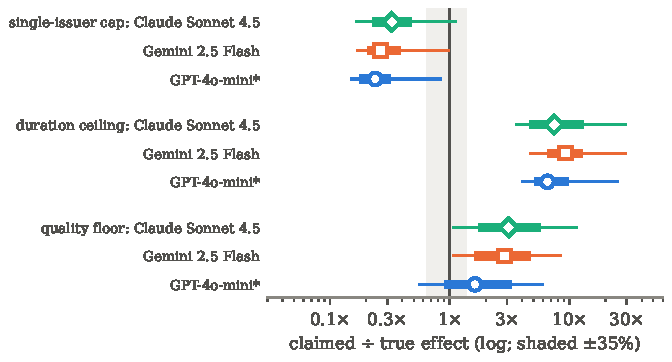
\includegraphics[width=\figw]{fig_v5_magnitude.pdf}
\caption{Claimed $\div$ true effect of relaxing each limit, per model
(median, interquartile range and 10th--90th percentile; log scale). The shaded
band is $\pm35\%$.}
\label{fig:mag}
\end{figure}

\subsection{Why the overall error rate understates the problem}
On the natural set, the share of explanations naming at least one zero-effect
limit was \hardMainSonFf\% for Claude and \hardMainGemFf\% for Gemini, against
\hardMainTmpl\% for the template. These rates look moderate only because most
limits bind in realistic problems, so naming every limit is usually right. The
conditional rates above show that the models do not discriminate: when a limit
does not matter, they usually cite it anyway.

\subsection{Copying the prompt's example}
\label{sec:anchor}
Our prompt ended with an example of the required output line containing the
values 12.0 (cap) and 4.5 (duration). GPT-4o-mini reproduced the 12.0 in
\anchorGpt\% of its answers, against \anchorGem\% for Gemini and \anchorSon\% for
Claude. Because its stated magnitudes largely restate the example, we exclude
GPT-4o-mini from the claims above. Its zero-effect rates are reported in full in
Table~\ref{tab:main}: 59\% with the basic prompt and 37\% with the facts, the
lowest of any LLM condition. Even at that rate, more than one in three limits
with no effect was cited as a driver.

\section{Discussion and Limitations}
\textbf{Implication.} An LLM asked to explain a constrained allocation from the
solution alone will usually produce a fluent account that cites limits with no
effect and misstates the costs of those that matter. Where the explanation
becomes a record, such as a committee paper, a client letter or an audit
response, this is a governance problem. Explanations generated from the
certificate avoid both errors by construction, which is consistent with the
design of tool-grounded systems~\cite{optiguide23,optichat25}. We did not test
whether an LLM that is given the certificate restates it faithfully. That
condition is the natural next experiment.

\textbf{Limitations.} (i) Assets are rating--maturity representative bonds
calibrated to public data, not individual securities, and the mandate has three
limits where real mandates have many more. (ii) The issuer cap bound in every
problem, so zero-effect attribution is measured for the duration and quality
limits only. (iii) The exact test relies on linear-programming duality. With
integer lot sizes or nonlinear objectives, shadow prices are no longer unique or
exact. Magnitudes are measured for a finite step and can understate the local
shadow price where a breakpoint is crossed (\S\ref{sec:method}). (iv) We evaluate
two models plus one reported separately, with one reply each at temperature 0.
Newer models, other sampling settings, reasoning modes or tool use (for example,
letting the model call a solver) may behave differently. (v) Our prompt contained
an example output line. We report its effect, and a neutral format line is a
natural refinement. (vi) The slack-focused set over-represents slack limits by
design, and we report the natural set alongside it.

\section{Conclusion}
For linear-programming portfolio decisions, the drivers of the decision are
known exactly, so explanations of those decisions can be checked exactly.
Checked this way, explanations written by two commercial LLMs without the
solver's certificate named limits with no effect as drivers in most of the
cases where that error was possible, while naming binding limits only somewhat
more often, and they stated the cost of binding limits within $\pm35\%$ in only
\magMain\% of claims. In settings where an explanation becomes a record, its
reasons should come from the certificate rather than from the model's reading of
the portfolio.
